\section{評価}\label{section:評価}
\subsection{Web APIの有用性}\label{subsection:PWAにおけるWeb APIの有用性}
\subsubsection{メディアの制御}\label{subsubsection:メディアの制御}
メディアを制御するWeb APIのWebブラウザーの対応状況を表~\ref{table:メディアを制御するWeb APIの対応状況}に示す。そのWeb APIに対するベンダーの意見を表~\ref{table:メディアを制御するWeb APIに対する意見}に示す。
\begin{table}
  \caption{メディアを制御するWeb APIの対応状況}
  \label{table:メディアを制御するWeb APIの対応状況}
  \centering
  \begin{tabular}{|p{13em}|p{8em}|p{8em}|}
    \hline
    & Google Chrome & Mozilla Firefox \\ \hline
    Media Capture and Streams API & 対応 & 対応 \\ \hline
    MediaStream Recording API & 対応 & 対応 \\ \hline
    Media Session API & 対応 & 対応 \\ \hline
    Encrypted Media Extensions API & 対応 & 対応 \\ \hline
    Media Stream Image Capture API & 対応 & 対応 \\ \hline
    Media Capabilities API & 対応 & 対応 \\ \hline
    Media Source Extensions API & 対応 & 対応 \\ \hline
  \end{tabular}
\end{table}
\begin{table}
  \caption{メディアを制御するWeb APIに対する意見}
  \label{table:メディアを制御するWeb APIに対する意見}
    \centering
    \begin{tabular}{|p{13em}|p{13em}|p{13em}|}
        \hline
        & Mozilla & WebKit \\ \hline
        Media Capture and Streams API & & \\ \hline
        MediaStream Recording API & & \\ \hline
        Media Session API & & \\ \hline
        Encrypted Media Extensions API & & \\ \hline
        Media Stream Image Capture API & & \\ \hline
        Media Capabilities API & & \\ \hline
        Media Source Extensions API & & \\ \hline
    \end{tabular}
\end{table}
Media Capture and Streams APIはカメラによるストリーミングを提供する。MediaStream Recording APIと組み合わせることで、音声や動画のストリーミングを収録できる。これらのAPIを活用すると、画面共有やビデオ通話といった機能を簡単に実装できる。Media Stream Image Capture APIと組み合わせることで写真を撮影することもできる。

MozillaやWebKitはこれらのAPIに肯定的である。getUserMedia()によってカメラやマイクへの明示的なアクセス許可を求められるため、ユーザーが処理の流れを理解しやすい点や、再生ボタンをクリックするなどのアクションに関連付けられている点で挙動が明確である。
\subsubsection{モジュールへのアクセス}\label{subsubsection:モジュールへのアクセス}
モジュールにアクセスするWeb APIのWebブラウザーの対応状況を表~\ref{table:モジュールにアクセスするWeb APIの対応状況}に示す。そのWeb APIに対するベンダーの意見を表~\ref{table:モジュールにアクセスするWeb APIに対する意見}に示す。
\begin{table}
  \caption{モジュールにアクセスするWeb APIの対応状況}
  \label{table:モジュールにアクセスするWeb APIの対応状況}
  \centering
  \begin{tabular}{|p{13em}|p{8em}|p{8em}|}
    \hline
    & Google Chrome & Mozilla Firefox \\ \hline
    Geolocaion API & \cellcolor{green!25}対応 & \cellcolor{green!25}対応 \\ \hline
    Web Bluetooth API & \cellcolor{green!25}対応 & \cellcolor{red!25}非対応 \\ \hline
    Screen Orientation API & \cellcolor{green!25}対応 & \cellcolor{red!25}非対応 \\ \hline
    Vibration API & \cellcolor{green!25}対応 & \cellcolor{green!25}対応 \\ \hline
  \end{tabular}
\end{table}
\begin{table}
    \centering
    \caption{モジュールにアクセスするWeb APIに対する意見}
    \label{table:モジュールにアクセスするWeb APIに対する意見}
    \begin{tabular}{|p{13em}|p{13em}|p{13em}|}
         \hline
         & Mozilla & WebKit \\ \hline
         Geolocaion API &  &  \\ \hline
         Web Bluetooth API &  &  \\ \hline
         Screen Orientation API &  &  \\ \hline
         Vibration API &  &  \\ \hline
    \end{tabular}
\end{table}
Geolocation APIはユーザーの位置情報を取得する。ユーザーの位置を地図上にプロットしたり、ユーザーの位置情報を用いて、パーソナライズされた情報を表示したい場合に便利である。プライバシー上の理由から明示的なアクセス許可やHTTPS通信が必要である。
Web Bluetooth APIはBluetooth Low Energyの周辺機器に接続して操作する機能を提供する。しかし、WebアプリがBluetooth端末に接続する場合は、そのアプリがどのような意図でその端末に接続しようとしているのかが明確に定義できないため、潜在的な危険性が高いと指摘されている~\cite{MozillaWebBluetooth}。
\subsubsection{バックグラウンド処理}\label{subsubsection:バックグラウンド処理}
バックグラウンド処理を行うWeb APIのWebブラウザーの対応状況を表~\ref{table:バックグラウンド処理を行うWeb APIの対応状況}に示す。そのWeb APIに対するベンダーの意見を表~\ref{table:バックグラウンド処理を行うWeb APIに対する意見}に示す。
\begin{table}
  \caption{バックグラウンド処理を行うWeb APIの対応状況}\label{table:バックグラウンド処理を行うWeb APIの対応状況}
  \centering
  \begin{tabular}{|p{13em}|p{8em}|p{8em}|}
    \hline
    & Google Chrome & Mozilla Firefox \\ \hline
    Background Tasks API & \cellcolor{green!25}対応 & \cellcolor{green!25}対応 \\ \hline
    Background Fetch API & \cellcolor{green!25}対応 & \cellcolor{red!25}非対応 \\ \hline
    Background Synchronization API & \cellcolor{green!25}対応 & \cellcolor{red!25}非対応 \\ \hline
    Web Workers API & \cellcolor{green!25}対応 & \cellcolor{green!25}対応 \\ \hline
  \end{tabular}
\end{table}
\begin{table}
  \caption{バックグラウンド処理を行うWeb APIに対する意見}
  \label{table:バックグラウンド処理を行うWeb APIに対する意見}
    \centering
    \begin{tabular}{|p{13em}|p{13em}|p{13em}|}
        \hline
        & Mozilla & WebKit \\ \hline
        Background Tasks API & & \\ \hline
        Background Fetch API & & \\ \hline
        Background Synchronization API & & \\ \hline
        Web Workers API & & \\ \hline
    \end{tabular}
\end{table}
Background Tasks APIはタスクをキューに入れて優先度が高いものから順番に実行する。キューに入れられたタスクはバックグラウンドで実行されるため、Web Workerを使用せずにシステムの遅延を削減できる長所がある。Background Fetch APIは大容量のファイルをバックグラウンドでフェッチする。オフラインでフェッチリクエストが実行された場合は、ユーザーが再びオンラインになるまでプロセスを一時停止させることもできる。Background Fetch APIが実行する処理は実質的にはバックグラウンドでのダウンロードやアップロードであり、それらの処理の後にスクリプトがバックグラウンドで実行される可能性がある。ユーザーの明示的な操作を必須にすることや、Background Fetch APIがSame-Originのコンテンツのみを扱えるように制限するべきであるという声もある。Background Synchronization APIは安定したネットワーク接続が確立されるまでタスクを延期する。このAPIを使用して延期されたタスクは、異なるネットワーク上で実行される可能性があるため、ユーザーが意図しない処理が行われることが懸念されている。
\subsubsection{ファイルへのアクセス}\label{subsubsection:ファイルへのアクセス}
ファイルにアクセスするWeb APIのWebブラウザーの対応状況を表~\ref{table:ファイルにアクセスするWeb APIの対応状況}に示す。そのWeb APIに対するベンダーの意見を表~\ref{table:ファイルにアクセスするWeb APIに対する意見}に示す。
\begin{table}
  \caption{ファイルにアクセスするWeb APIの対応状況}\label{table:ファイルにアクセスするWeb APIの対応状況}
  \centering
  \begin{tabular}{|p{13em}|p{8em}|p{8em}|}
    \hline
    & Google Chrome & Mozilla Firefox \\ \hline
    File API & \cellcolor{green!25}対応 & \cellcolor{green!25}対応 \\ \hline
    File System Access API & \cellcolor{green!25}対応 & \cellcolor{green!25}対応 \\ \hline
    File System API & \cellcolor{green!25}対応 & \cellcolor{green!25}対応 \\ \hline
    File and Directory Entries API & \cellcolor{green!25}対応 & \cellcolor{green!25}対応 \\ \hline
  \end{tabular}
\end{table}
\begin{table}
  \caption{ファイルにアクセスするWeb APIに対する意見}
  \label{table:ファイルにアクセスするWeb APIに対する意見}
    \centering
    \begin{tabular}{|p{13em}|p{13em}|p{13em}|}
        \hline
        & Mozilla & WebKit \\ \hline
        File API & & \\ \hline
        File System Access API & & \\ \hline
        File System API & & \\ \hline
        File and Directory Entries API & & \\ \hline
    \end{tabular}
\end{table}
File APIは端末のファイルとそのコンテンツにアクセスする。File APIよりも汎用性が高いAPIとしてはFile System Access APIがある。File System Access APIは端末のファイルシステム上のファイルにアクセスしてファイルを読み込んだり、ファイルに書き込んだりできる。File System APIはWebブラウザーに仮想ドライブを作成し、そのストレージにファイルを保存するものであり、File System APIとFile System Access APIはそれぞれ異なるAPIである。File System Access APIは端末のすべてのディレクトリとファイルにアクセスする権限を持つため、悪用されるリスクがある。許可を求めるプロンプトの表示などによって、このAPIが行おうとしている操作をユーザーに分かりやすく提示することで安全性を確保できるという意見もある。
\subsubsection{通知の制御}\label{subsubsection:通知の制御}
通知を制御するWeb APIのWebブラウザーの対応状況を表~\ref{table:通知を制御するWeb API}に示す。そのWeb APIに対するベンダーの意見を表~\ref{table:通知を制御するWeb APIに対する意見}に示す。
\begin{table}
  \caption{通知を制御するWeb API}\label{table:通知を制御するWeb API}
  \centering
  \begin{tabular}{|p{13em}|p{8em}|p{8em}|}
    \hline
    & Google Chrome & Mozilla Firefox \\ \hline
    Push API & \cellcolor{green!25}対応 & \cellcolor{green!25}対応 \\ \hline
    Push API & \cellcolor{green!25}対応 & \cellcolor{green!25}対応 \\ \hline
    Notifications API & \cellcolor{green!25}対応 & \cellcolor{green!25}対応 \\ \hline
    Badging API & \cellcolor{green!25}対応 & \cellcolor{red!25}非対応 \\ \hline
  \end{tabular}
\end{table}
\begin{table}
  \caption{通知を制御するWeb APIに対する意見}
  \label{table:通知を制御するWeb APIに対する意見}
    \centering
    \begin{tabular}{|p{13em}|p{13em}|p{13em}|}
        \hline
        & Mozilla & WebKit \\ \hline
        Push API & & \\ \hline
        Notifications API & & \\ \hline
        Badging API & & \\ \hline
    \end{tabular}
\end{table}
Push APIはWebアプリがサーバーからプッシュ通知を受信する機能を提供する。Webアプリがフォアグラウンドで動作していなくても利用できるため、任意のイベントを通知してユーザーの関心を集められる。WebアプリからOSなどのシステムに対して通知を送るためにはNotifications APIを用いる。Badging APIを併用することで通知の数などの状態が変化したことをユーザーに通知できる。Notifications APIとBadging APIは、HTTPSでサーバーと通信しており、かつService WorkerなどのWebワーカーが動作しているWebアプリでのみ利用できる。
\subsection{Service Workerのパフォーマンス}\label{subsubsection:Service Workerのパフォーマンス}
Lighthouseとネットワークスロットリングを使用して、それぞれの都道府県の観光地図を読み込んだ際のパフォーマンスを計測した。パフォーマンスを計測する際に使用したネットワークスロットリングのプロファイルを表~\ref{table:ネットワークスロットリングのプロファイル}に示す。キャッシュ戦略ごとのそれぞれの指標の測定値の平均を図~\ref{figure:Service Workerを使用しなかった場合のパフォーマンス}、~\ref{figure:全てのネットワークレスポンスをキャッシュした場合のパフォーマンス}、~\ref{figure:画像をキャッシュした場合のパフォーマンス}、~\ref{figure:Same-Originのネットワークレスポンスをキャッシュした場合のパフォーマンス}に示す。

\begin{table}
  \caption{ネットワークスロットリングのプロファイル}\label{table:ネットワークスロットリングのプロファイル}
  \centering
  \begin{tabular}{|p{5em}|p{10em}|p{10em}|p{10em}|}
    \hline
    & アップリンク[Kbit/s] & ダウンリンク[Kbit/s] & RTT[ms] \\ \hline
    3gslow & 400 & 400 & 200 \\ \hline
    3gfast & 768 & 1600 & 75 \\ \hline
    4g & 9000 & 9000 & 85 \\ \hline
  \end{tabular}
\end{table}

\begin{figure}
  \centering
  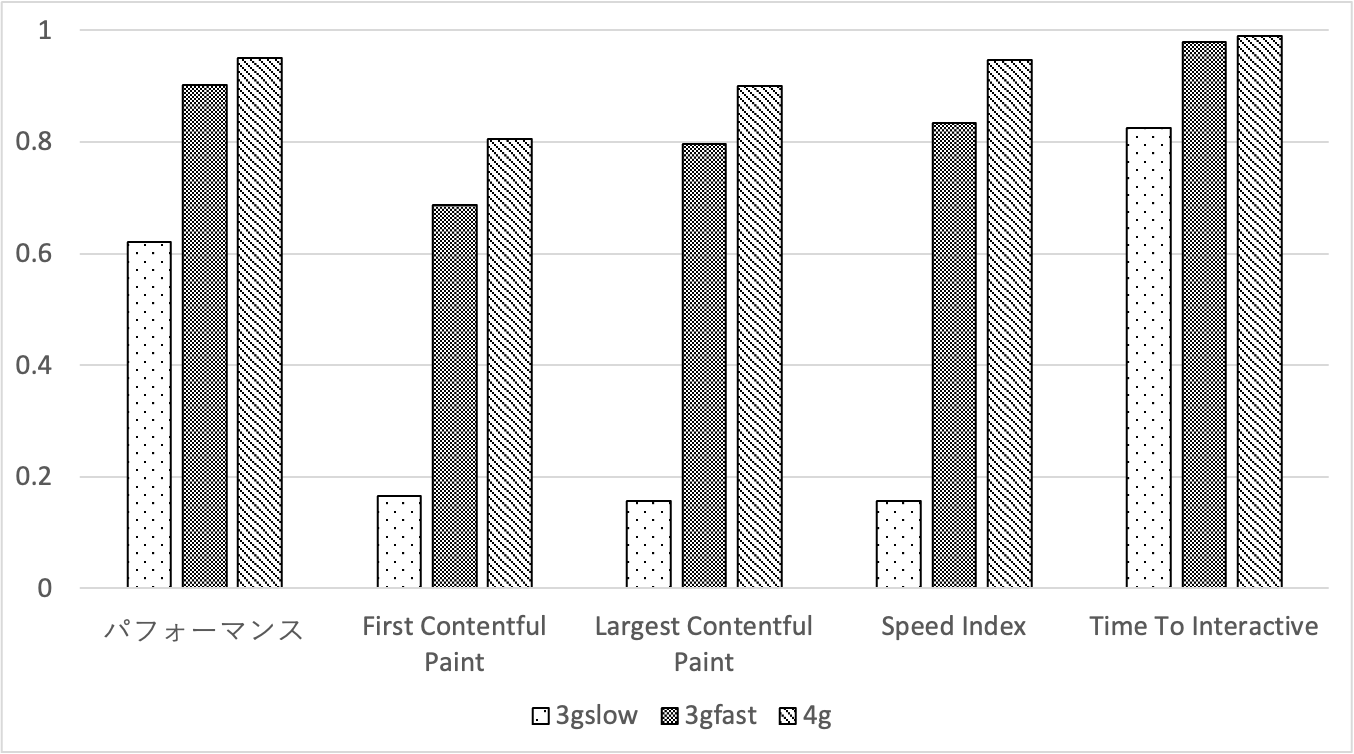
\includegraphics[width=0.9\textwidth]{images/without_service_worker.png}
  \caption{Service Workerを使用しなかった場合のパフォーマンス}\label{figure:Service Workerを使用しなかった場合のパフォーマンス}
\end{figure}

\begin{figure}
  \centering
  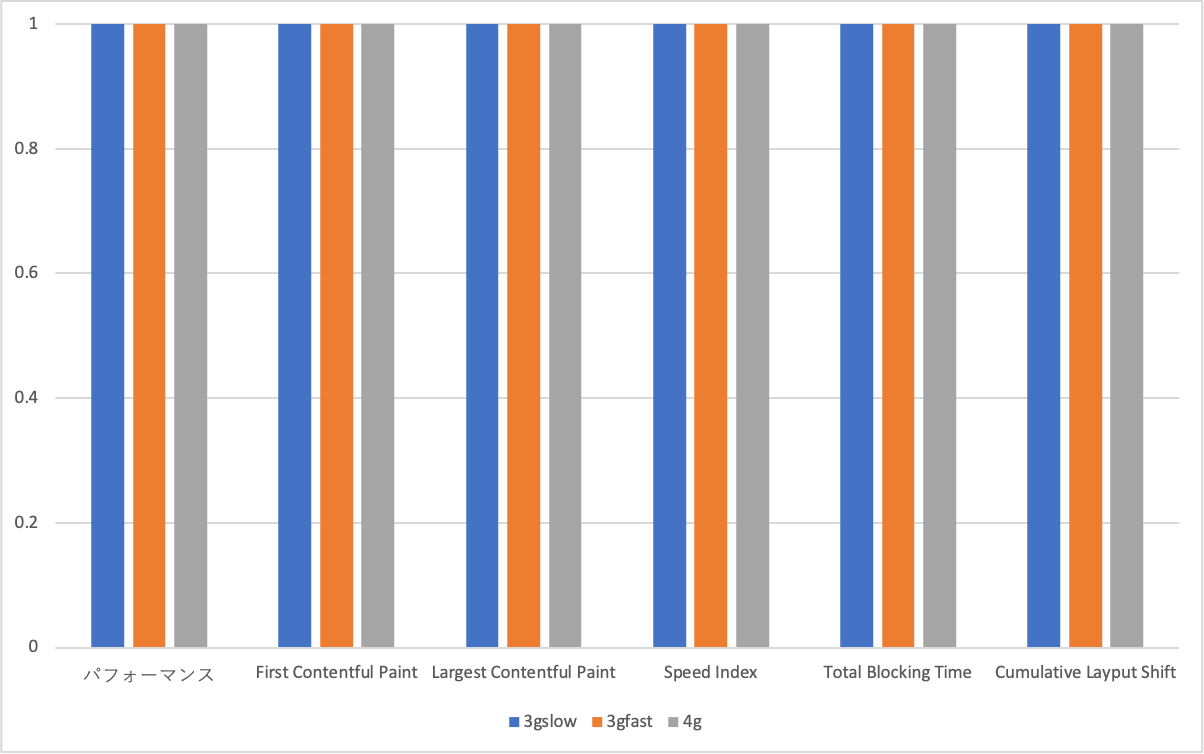
\includegraphics[width=0.9\textwidth]{images/service_worker_cache_all.png}
  \caption{全てのネットワークレスポンスをキャッシュした場合のパフォーマンス}\label{figure:全てのネットワークレスポンスをキャッシュした場合のパフォーマンス}
\end{figure}

\begin{figure}
  \centering
  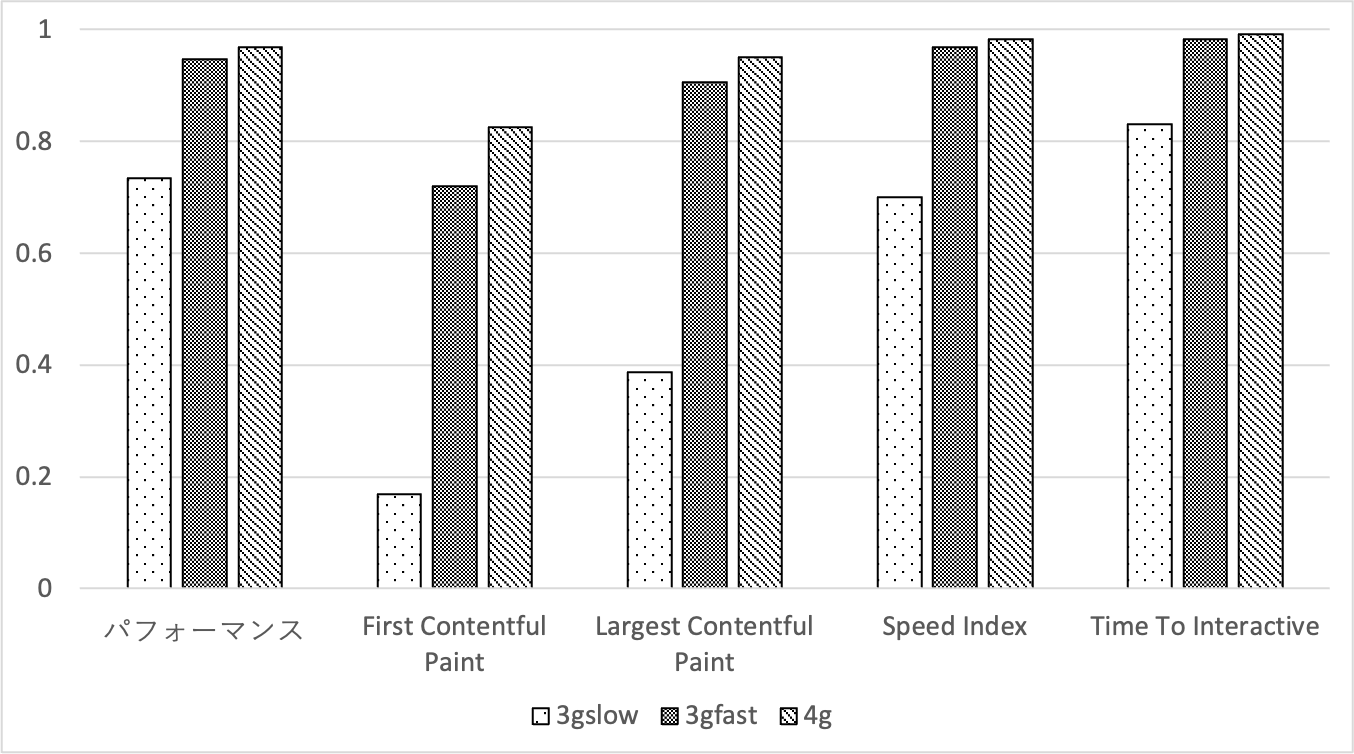
\includegraphics[width=0.9\textwidth]{images/service_worker_cache_images.png}
  \caption{画像をキャッシュした場合のパフォーマンス}\label{figure:画像をキャッシュした場合のパフォーマンス}
\end{figure}

\begin{figure}
  \centering
  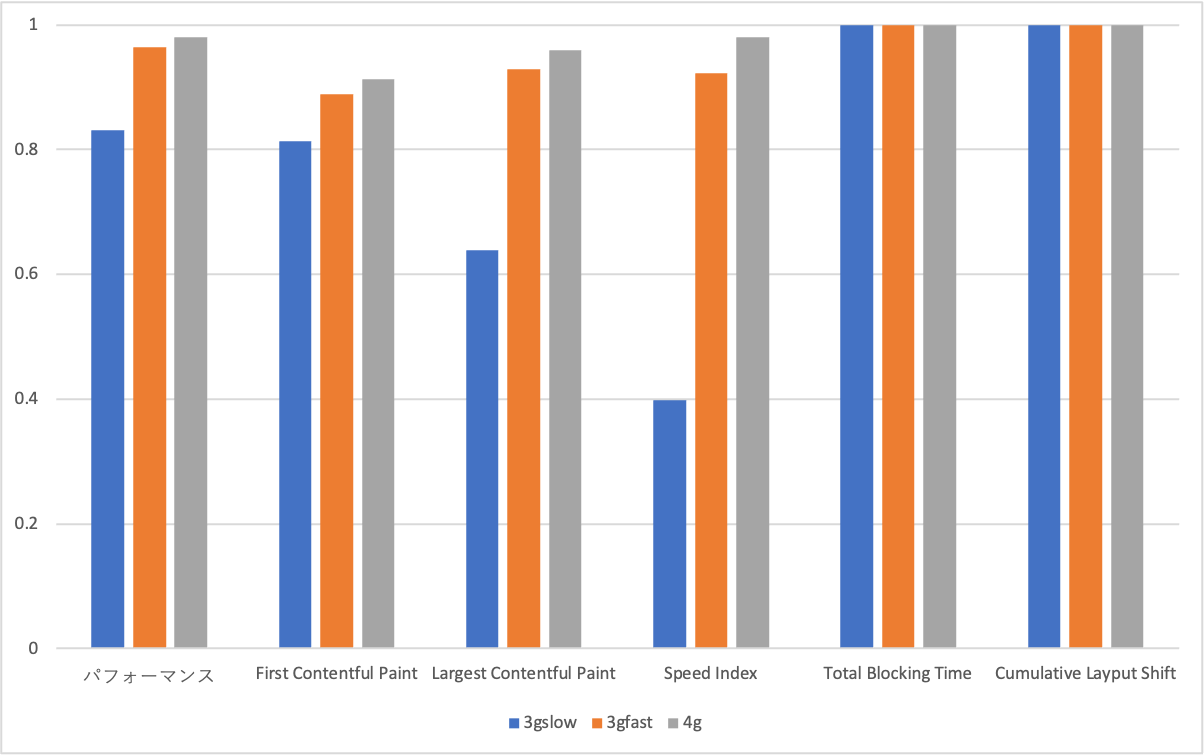
\includegraphics[width=0.9\textwidth]{images/service_worker_cache_same_origin.png}
  \caption{Same-Originのネットワークレスポンスをキャッシュした場合のパフォーマンス}\label{figure:Same-Originのネットワークレスポンスをキャッシュした場合のパフォーマンス}
\end{figure}

いずれの場合もTBTとCLSは1である。4g、3gfast、3gslowの順でパフォーマンスの指標の値が大きい傾向にある。全てのネットワークレスポンスをキャッシュした場合は3gslow、3gfast、4gのいずれの場合も全ての指標の値は1である。画像をキャッシュした場合はFCPが最も通信速度の低下の影響を受けやすく、SIが最もその影響を受けにくいことが分かる。逆に、Same-Originのネットワークレスポンスのキャッシュした場合はSIが最も通信速度の低下の影響を受けやすく、SCPが最もその影響を受けにくいことが示されている。

3gfastに比べてアップリンクがおよそ12倍、ダウンリンクがおよそ6倍である4gプロファイルを使用した場合であってもほとんどのパフォーマンスの指標の値は1未満である。全体的に見ると、3gslowと3gfast間のパフォーマンス指標の値の増加率は3gfastと4g間の増加率よりも大きい。